\section{\method: A Language-Grounded Semantic Interface for Accident Anticipation}
\label{sec:method}

We present \method{}, a framework whose central object is a
\emph{language-grounded risk concept interface}. The interface is built first
through a reproducible ontology pipeline and then used as the semantic
bottleneck of an interpretable anticipation model. Figure~\ref{fig:framework}
summarizes the full system.
This design follows the information-bottleneck principle in that a constrained,
named intermediate space is explicitly optimized for downstream utility while
remaining inspectable to users and protocol designers~\citep{tishby2000information}.

\begin{figure*}[t]
  \centering
  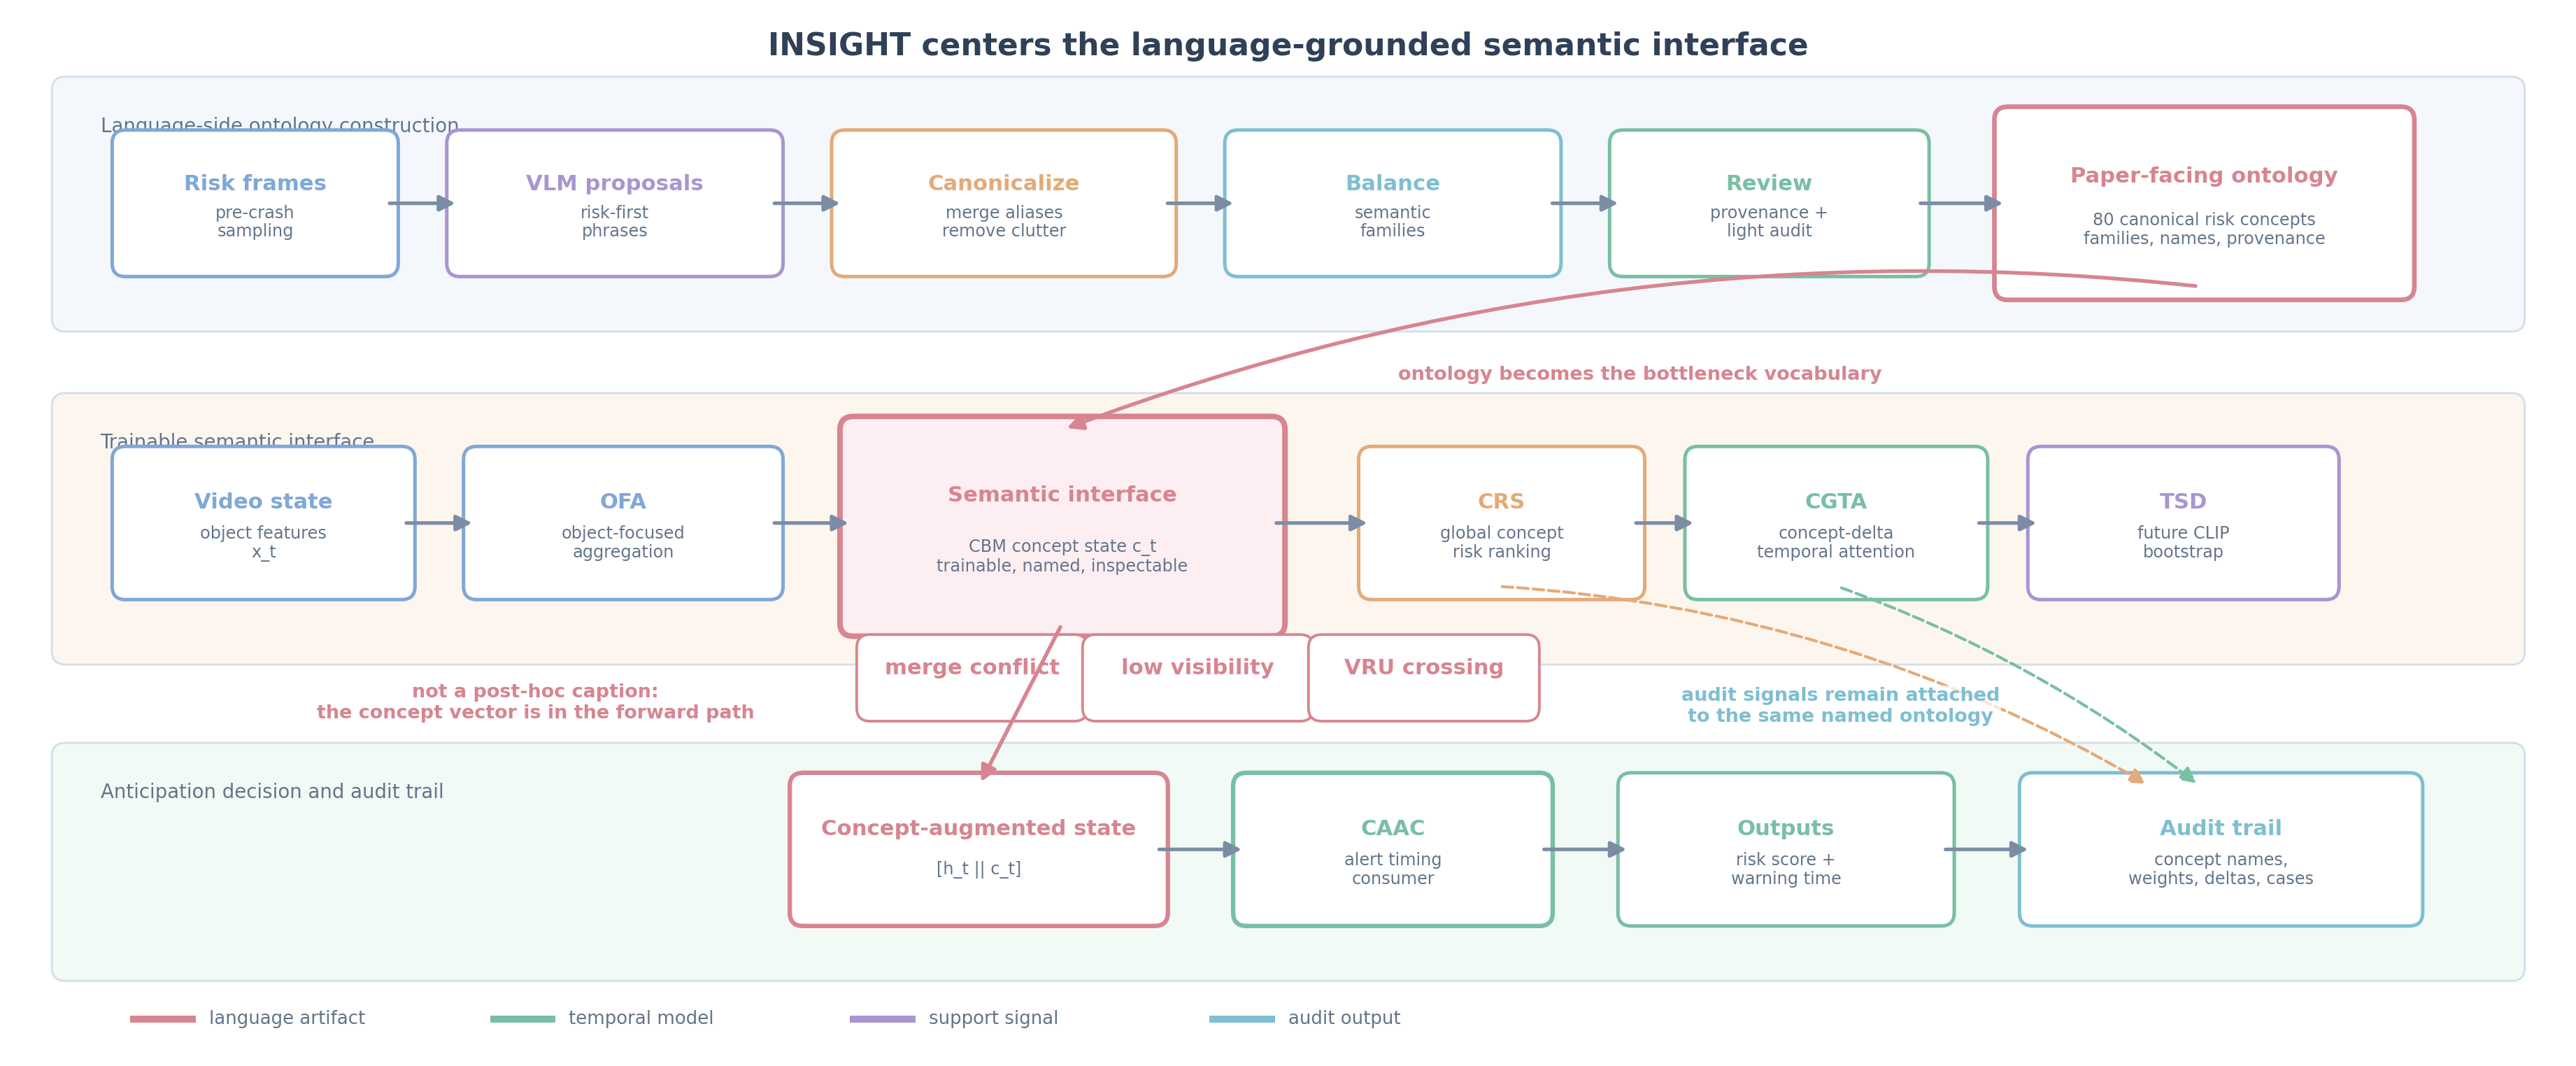
\includegraphics[width=\textwidth]{../figures/insight_framework.pdf}
  \caption{\textbf{\method{} as a semantic-interface pipeline.}
  Per-frame object features are aggregated, mapped into an explicit concept
  space, and then consumed by downstream anticipation modules. In this paper,
  the most important object is the semantic interface:
  the ontology construction pipeline produces the concepts, the CBM exposes
  them as trainable state, CRS and CGTA make them auditable over time, and the
  timing module consumes them as part of its decision state.}
  \label{fig:framework}
\end{figure*}

\subsection{Problem Setup and Design Scope}

Given a dashcam video $\{\mathbf{x}_t\}_{t=1}^T$ with
$\mathbf{x}_t \in \mathbb{R}^{N \times D}$, a binary label
$y \in \{0,1\}$, and time-of-accident $\tau$, accident anticipation is usually
framed as predicting whether an accident will occur from a video prefix. Our
goal is more specific: to expose a semantic interface that allows the model's
risk evidence to be named, compared, and audited while retaining competitive
predictive behavior.

We use the following idealized objective as a motivating target:
\begin{equation}
  \max_{\theta}\; \mathbb{E}[\mathrm{TTA}]
  \quad \text{s.t.} \quad \mathrm{AP}(\theta) \geq \mathrm{AP}_{\text{base}},
  \label{eq:objective}
\end{equation}
where TTA is the warning lead time and AP is the standard precision--recall
metric. This equation simply states the target operating regime: improve lead
time without sacrificing predictive quality. Our methodological contribution is
the semantic interface that lets us study how ontology design changes this
operating point.

\subsection{Ontology Construction as Method}

\paragraph{Why ontology construction belongs in the method section.}
A concept bottleneck is only as useful as the concept vocabulary it exposes.
In accident anticipation, a generic traffic lexicon is often too broad, while
a fully manual ontology is difficult to scale and hard to govern
systematically. We therefore treat ontology construction as part of the method
rather than as hidden preprocessing. The aim is to produce \emph{trainable,
auditable, and comparable} risk primitives rather than a loose list of scene
descriptions.

\paragraph{Stage 1: risk-oriented frame mining.}
We first sample pre-crash frames from positive videos to cover diverse traffic
geometries, actor interactions, visibility conditions, and accident precursor
patterns. Sampling is intentionally risk-oriented: the goal is to expose
emerging hazards rather than to maximize generic visual diversity. This reduces
annotation cost while preserving the semantic support needed for downstream
concept discovery.

\paragraph{Stage 2: multimodal risk concept proposal.}
Given the sampled frames, a multimodal model proposes candidate concepts,
risk factors, and coarse semantic families. Our prompts ask explicitly for
\emph{risk-first} concepts, such as cut-in behavior, closing distance,
visibility degradation, or vulnerable-road-user interaction, instead of generic
scene captions. The output of this stage is a noisy but high-recall pool of
candidate accident precursors.

\paragraph{Stage 3: risk-first refinement and canonical merge.}
The raw candidate pool is then refined into reusable risk primitives. We
prioritize risk-relevant or precursor-like factors, remove obvious
background clutter, merge near-duplicates, and normalize phrasing toward short
canonical names. This step is not merely cosmetic. Stable downstream training
benefits more from reusable concepts than from many near-synonymous
micro-labels, so the refinement policy intentionally favors semantic stability
over maximal lexical granularity.

\paragraph{Stage 4: family balancing and light human review.}
The ontology is further polished through family-level coverage auditing,
duplicate-cluster consolidation, and a light human review pass. The result is a
\emph{paper-facing semantic interface}: compact enough to present clearly, rich
enough to retain major accident precursor families, and explicit enough to
support provenance tracking, case studies, and matched ontology comparisons.

\paragraph{Stage 5: export as a trainable research asset.}
The final ontology is stored with canonical concept names, family metadata,
merge provenance, and review notes. This matters because the ontology is not
used only for figures. It is encoded and deployed as the actual bottleneck
vocabulary of the model, so ontology construction is evaluated not just by
semantic plausibility but by whether the resulting interface survives contact
with downstream learning.

\paragraph{What makes the interface language-grounded and governed.}
The paper's claim does not rest on any single multimodal model being perfectly
right about frame semantics. It rests on a governed language layer: prompts are
risk-oriented, outputs are canonicalized into short stable names, semantic
families are balanced explicitly, and retained concepts carry provenance and
review metadata. This matters because the scientific question is not only
whether concepts can be proposed, but whether the resulting ontology is stable
enough to function as a named interface between visual evidence and downstream
anticipation behavior.

\begin{figure*}[t]
  \centering
  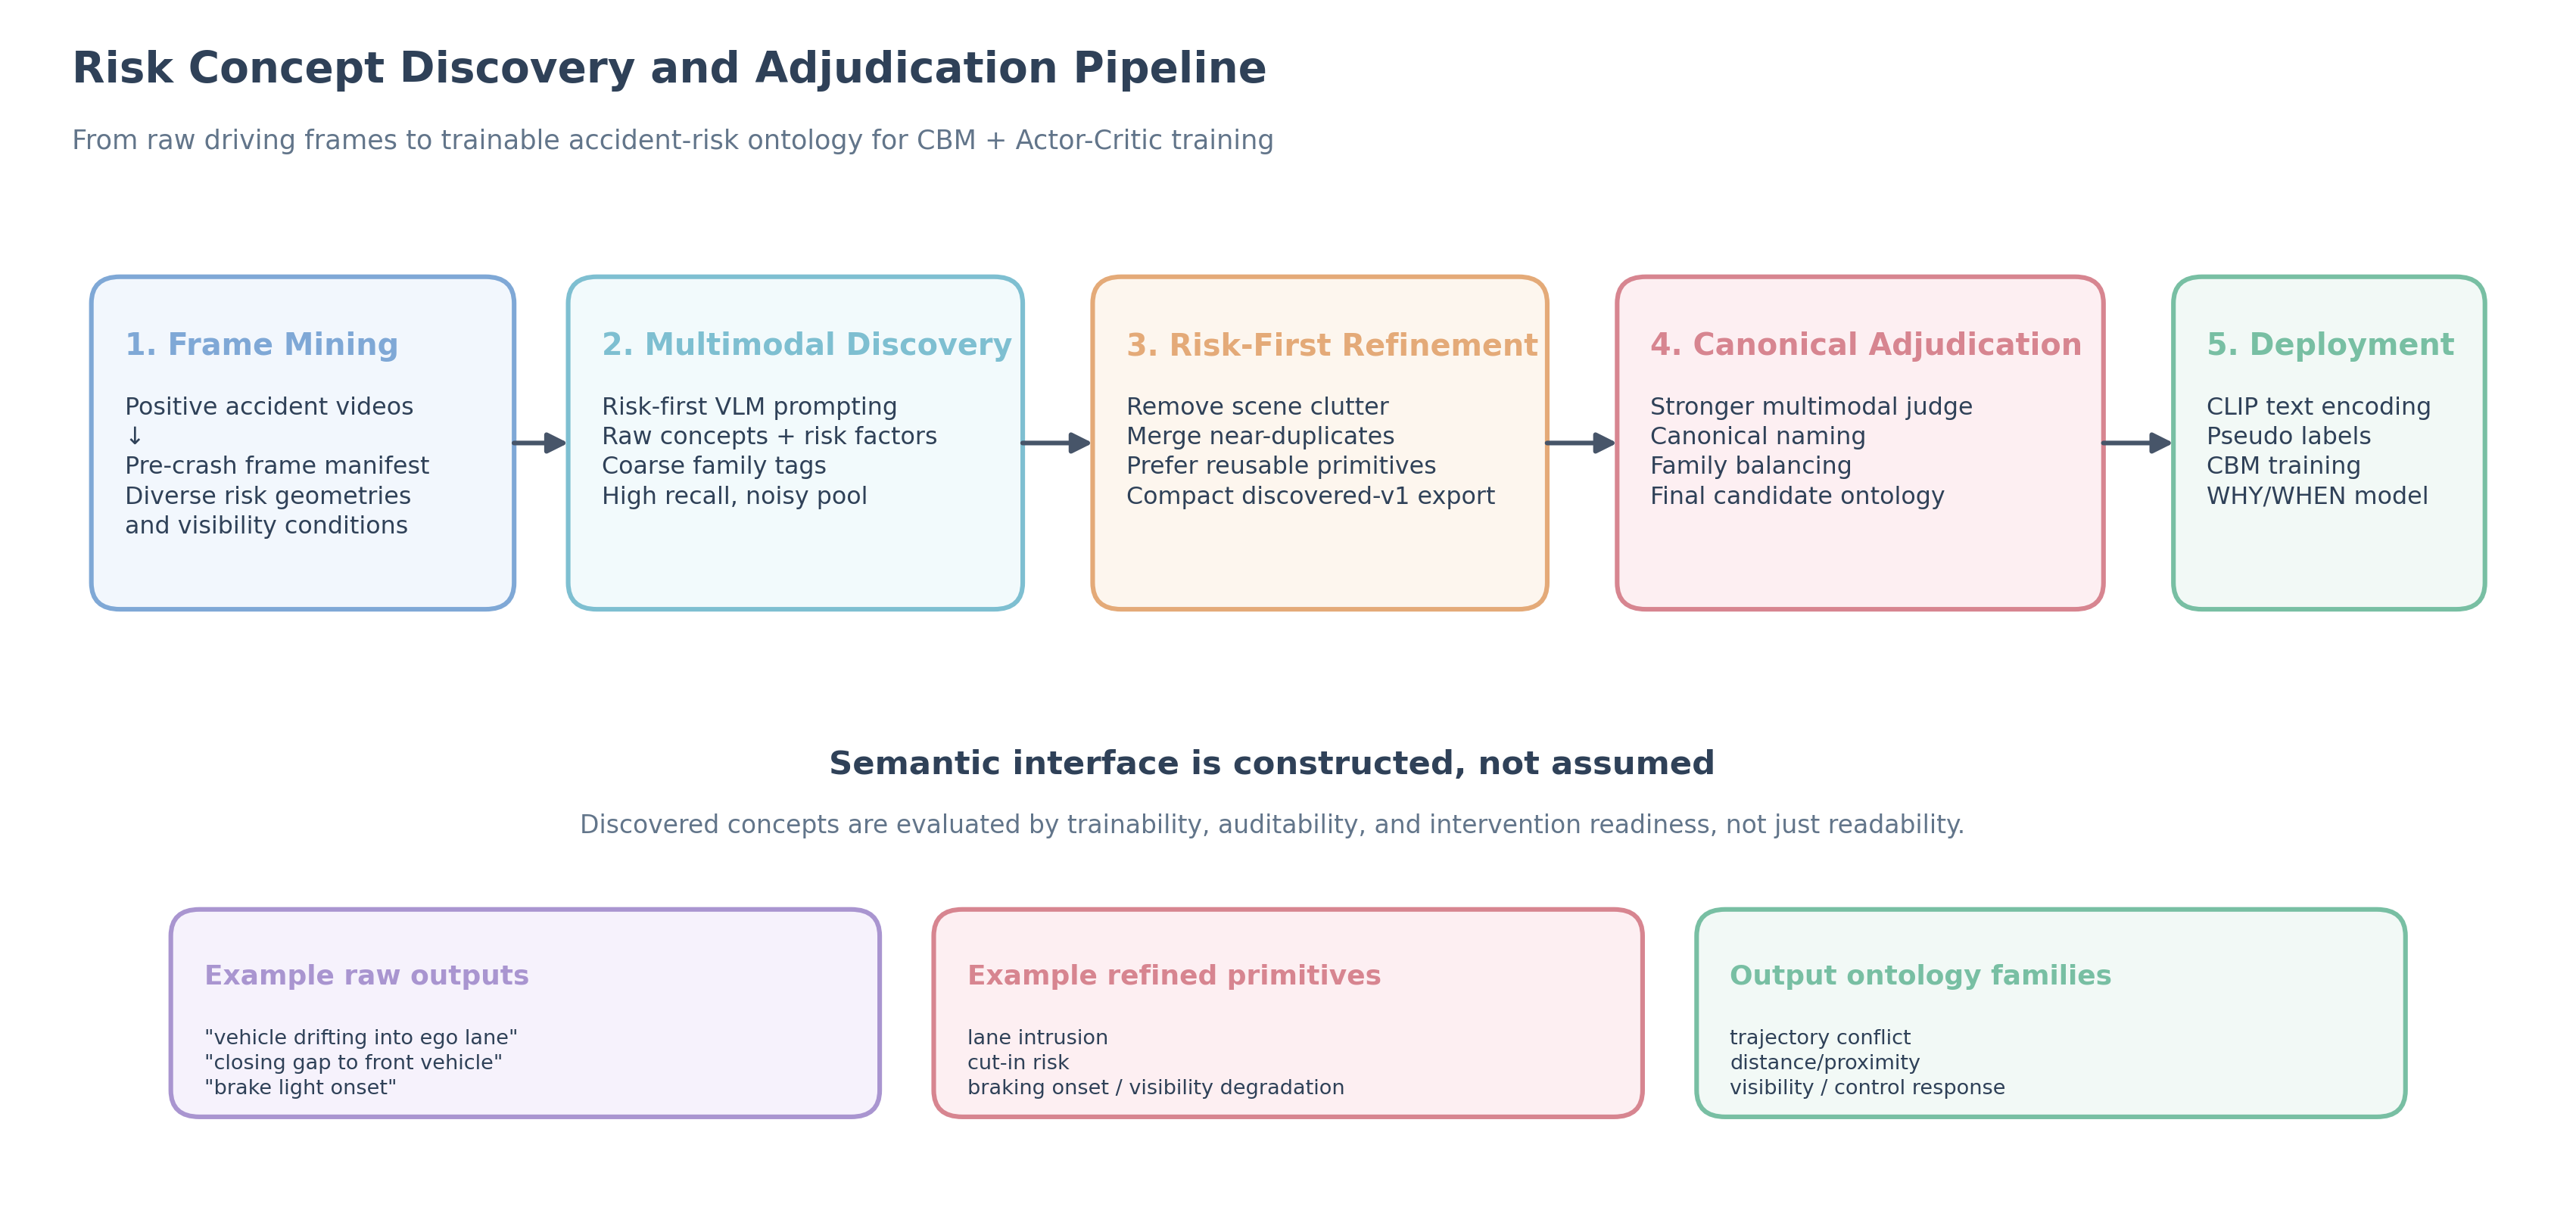
\includegraphics[width=0.98\textwidth]{../figures/insight_fig_concept_pipeline.pdf}
  \caption{\textbf{End-to-end risk ontology construction.}
  Starting from sampled pre-crash frames, the pipeline performs multimodal
  concept proposal, risk-first refinement, duplicate consolidation, family
  balancing, and light human review to produce a trainable ontology for the
  concept bottleneck. The ontology is therefore a reproducible methodological
  component rather than a hidden vocabulary assumption.}
  \label{fig:concept_pipeline}
\end{figure*}

\subsection{Model Overview}

Once the ontology is fixed for a run, \method{} uses it as the semantic
bottleneck of the anticipation model. The per-frame forward pass is
\begin{align*}
  \mathbf{x}_t
  &\xrightarrow{\text{OFA}} \mathbf{o}_t
  \xrightarrow{\cbm} (\mathbf{c}_t,\mathbf{e}_t)
  \xrightarrow{\crs} \rho_t \\
  &\xrightarrow{\cgta} \mathbf{g}_t
  \xrightarrow{\text{GRU}} \mathbf{h}_t
  \xrightarrow{\caac} (p_t, a_t, V_t).
\end{align*}
The key design choice is that downstream anticipation does not consume only an
opaque hidden state. It also consumes the explicit concept activations
$\mathbf{c}_t$, which makes the system's semantic interface available to both
prediction and timing.

\subsection{Object-Focused Aggregation}

Each frame contains $N$ object features. We aggregate them through
Object-Focused Attention (OFA):
\begin{align}
  \alpha^n_t &= \mathrm{softmax}_n\bigl(\mathbf{w}_a^\top
    \tanh(\mathbf{W}_o \mathbf{x}^n_t)\bigr), \\
  \mathbf{o}_t &= \sum_{n=1}^N \alpha^n_t\,\mathbf{W}_f \mathbf{x}^n_t.
\end{align}
This provides a compact frame representation that preserves actor-level
salience before the semantic bottleneck is applied.

\subsection{Concept Bottleneck Module}

The Concept Bottleneck Module maps the aggregated frame representation to
$K$ interpretable risk concepts, where $K$ depends on the ontology used in the
run ($K{=}837$ for the historical full set and smaller values for compact
ontologies):
\begin{align}
  \mathbf{c}_t &= \sigma(\mathbf{W}_c \mathbf{o}_t + \mathbf{b}_c)
    \in [0,1]^K, \\
  \mathbf{e}_t &= \mathrm{LayerNorm}(\mathbf{W}_d \mathbf{c}_t + \mathbf{b}_d).
\end{align}
The vector $\mathbf{c}_t$ is the paper's strongest interpretability object:
each dimension corresponds to a named risk concept in the ontology.

\paragraph{Pseudo-label supervision.}
We supervise the bottleneck with CLIP-derived pseudo-labels
$\hat{\mathbf{c}}_t \in \{0,1\}^K$. For each frame, a concept is marked
positive if its similarity score lies in the frame-wise top-$m$ set
($m{=}3$ in the main recipe). The auxiliary loss is
\begin{equation}
  \mathcal{L}_{\text{aux}}
  = \frac{1}{K}\,\mathrm{BCE}(\mathbf{c}_t,\,\hat{\mathbf{c}}_t).
\end{equation}
We interpret these pseudo-labels as a semantic bootstrap rather than as a claim
of perfect concept correctness.

\subsection{Concept Risk Score and Temporal Semantic Modeling}

\paragraph{Concept Risk Score (CRS).}
To expose a global audit signal, we learn per-concept risk weights
$\mathbf{w}_{\text{risk}} \in \mathbb{R}^K$ and compute
\begin{equation}
  \rho_t = \sigma(\mathbf{w}_{\text{risk}})^\top \mathbf{c}_t.
  \label{eq:crs}
\end{equation}
Unlike attention weights that vary from case to case, CRS provides a global
ranking that can be inspected as part of the semantic interface. In the current
paper, however, we treat CRS as an audit-oriented support signal rather than as
a fully mature standalone product claim.

\paragraph{Concept-Guided Temporal Attention (CGTA).}
Standard temporal attention is often difficult to interpret. We instead drive
temporal attention with concept deltas so that changes in semantic state guide
where the model looks in history:
\begin{align}
  \Delta\mathbf{c}_t &= \mathbf{c}_t - \mathbf{c}_{t-1}, \\
  \alpha_{t,s} &=
    \frac{\exp\bigl((\mathbf{W}_Q\Delta\mathbf{c}_t)^\top
      (\mathbf{W}_K\mathbf{h}_s)/\sqrt{h}\bigr)}
    {\sum_{s'=1}^{t-1}\exp\bigl((\mathbf{W}_Q\Delta\mathbf{c}_t)^\top
      (\mathbf{W}_K\mathbf{h}_{s'})/\sqrt{h}\bigr)}, \\
  \mathbf{g}_t &= \lambda_{\text{gate}}\sum_{s=1}^{t-1}\alpha_{t,s}\mathbf{W}_V\mathbf{h}_s
    + (1-\lambda_{\text{gate}})\mathbf{h}_{t-1}.
\end{align}
When a risk concept spikes, CGTA highlights the historical frames that likely
caused the change, creating a temporal audit trail for the semantic layer.

\subsection{Temporally Shifted Distillation}

To inject anticipatory information into the hidden representation, we distill
future CLIP features into the current state:
\begin{equation}
  \mathcal{L}_{\text{TSD}}
  = \bigl\|\mathbf{W}_{\text{TSD}}\mathbf{o}_t
    - \mathrm{sg}(\mathbf{f}^{\text{CLIP}}_{t+\delta})\bigr\|_2^2,
  \label{eq:tsd}
\end{equation}
where $\delta{=}5$ frames and $\mathrm{sg}(\cdot)$ denotes stop-gradient.
TSD is a support module: it encourages the model to encode where the scene is
headed, while the paper's main scientific focus remains the semantic interface
that drives downstream anticipation.

\subsection{Concept-Conditioned Timing Module}

\paragraph{Why timing still matters in this paper.}
Although this paper centers the semantic interface, accident
anticipation remains a temporal decision problem. The role of the timing module
is therefore to consume the concept state and expose how semantic evidence
shapes warning behavior. In the experiments, semantic-layer and ontology
comparisons carry the central claim, while actor-policy timing is reported as a
downstream transfer test of that interface.

\paragraph{State.}
The timing module consumes a concept-conditioned state
\begin{equation}
  \mathbf{s}_t = [\mathbf{h}_t \| \mathbf{c}_t].
  \label{eq:state}
\end{equation}
Architecturally, this is the crucial link from language-grounded concepts to
downstream temporal behavior: the timing module no longer acts on an opaque
latent vector alone.

\paragraph{Actor and Critic.}
The actor-critic formulation follows a standard policy-optimization setup
\citep{konda1999actor,sutton2018reinforcement}.
We parameterize an actor and critic over the concept-conditioned state:
\begin{align}
  \pi(a_t \mid \mathbf{s}_t)
    &= \mathrm{Softmax}(\mathbf{W}_\pi \mathbf{s}_t + \mathbf{b}_\pi), \\
  V(\mathbf{s}_t)
    &= \mathbf{w}_V^\top \tanh(\mathbf{W}_{V_1}\mathbf{s}_t).
\end{align}

\paragraph{Reward.}
Each video is a finite-horizon episode. The reward favors early correct alerts
and penalizes false alarms and misses:
\begin{equation}
  \mathfrak{r}_t = \begin{cases}
    \begin{aligned}[t]
      \lambda_r \cdot \dfrac{\tau - t}{\tau}\\
      \cdot (1 + \beta\, b_t)
    \end{aligned}
      & \text{first positive alert, } t < \tau \\[4pt]
    -\lambda_p & \text{false alert or miss} \\[4pt]
    +\varepsilon & \text{wait before end}
  \end{cases}
  \label{eq:reward}
\end{equation}
where $b_t = \sigma(\mathbf{w}_b^\top \mathbf{c}_t)$ is a learnable concept
bonus. This term encourages the policy to favor early alerts that are backed by
strong concept evidence.

\paragraph{Actor-Critic objective and evaluation scope.}
With advantage $A_t = R_t - V(\mathbf{s}_t)$ and discounted return $R_t$, the
Actor-Critic loss is
\begin{align}
  \mathcal{L}_{\text{AC}}
  &= -\mathbb{E}_t[\log\pi(a_t\mid\mathbf{s}_t)\,A_t] \nonumber\\
  &\quad + \lambda_V \mathbb{E}_t[(V(\mathbf{s}_t)-R_t)^2] \nonumber\\
  &\quad - \lambda_H \mathcal{H}[\pi(\cdot\mid\mathbf{s}_t)].
  \label{eq:ac_loss}
\end{align}
In the current paper, the canonical headline AP/mTTA numbers are still derived
from the classifier trajectory rather than from a fully validated standalone
actor policy. We therefore use CAAC to test how much timing behavior transfers
to a concept-conditioned policy, while keeping the canonical predictive
headline on the classifier branch and avoiding stronger policy-level claims than
the current evidence supports.

\subsection{Total Training Objective}

The overall objective balances classification, concept supervision, timing
training, and anticipatory distillation:
\begin{equation}
  \mathcal{L}
  = \mathcal{L}_{\text{CE}}
  + \lambda_{\text{aux}}\,\mathcal{L}_{\text{aux}}
  + \lambda_{\text{AC}}\,\mathcal{L}_{\text{AC}}
  + \lambda_{\text{TSD}}\,\mathcal{L}_{\text{TSD}}.
  \label{eq:total_loss}
\end{equation}
We use a warmup-and-ramp schedule so that concept learning stabilizes before
the timing objective becomes dominant. This matters because the timing module
is only useful if the semantic state it consumes is already coherent.

\subsection{Design Rationale and Complexity Notes}
\label{sec:theory}

\paragraph{Complexity.}
The dominant costs come from the recurrent backbone and the concept-dependent
projections. With the current hidden sizes and ontology sizes, these costs
remain compatible with a 30M-parameter model. The practical point is modest but
important: exposing a semantic interface does not require the very large model
scale used by several recent non-interpretable anticipation systems.

\paragraph{Why intervention is structurally meaningful.}
If a concept edit $\Delta\mathbf{c}$ is applied before prediction, the timing
state becomes $\mathbf{s}'_t = [\mathbf{h}_t \| \mathbf{c}_t + \Delta\mathbf{c}]$.
This does not prove that every trained model will respond monotonically to
every edit. What it does show is that concept edits act on the same state
consumed by downstream timing. For this reason, the intervention studies in the
experiments section are meaningful as tests of a \emph{structurally
intervenable} interface, even though full policy-level causal validation lies
beyond the scope of the current paper.
